

\subsection{Image Representation}\label{sec:image-rep}
% For simplicity \marginpar{@avaswani: simplicity might not be the right way to say this}, we treat the pixel RGB intensities as categorical variables rather than real numbers, and each channel has a separate set of $256$ embedding vectors for intensity values $0-255$. After embedding lookup and flattening along the width dimension, 3-d images of height $\height$, width $\width$ and $3$ channels becomes 3-d tensors of shape $[\height, \width \times 3, \modeldim]$ where $\modeldim$ is the model dimension, for example $512$. To enable the model to compute distances in $2$ dimensions between pixels, we add separate $\height$ and $\width \times 3$ $d$-dimension positional encodings for each row and width position to the image. Following~\cite{aiayn}, use sines and cosines for our positional encodings. Our local 2-d attention models (Section~\ref{sec:loc-2d}) receive this position augmented tensor. For local 1-d attention (Section~\ref{sec:loc-1d}), and input to our super-resolution models, we flatten the image in raster scan order, similar to existing work (\cite{PixelCNNpp,PixelRNN,PixelCNN}), and feed the image as a $[\height \times \width \times 3, \modeldim]$ tensor.
% We treat the predicted pixel intensities of the output as categorical variables. 
We treat pixel intensities as either discrete categories or ordinal values; this setting depends on the distribution (Section \ref{sub:loss}).
For categories, each of the input pixels' three color channels is encoded using a channel-specific set of $256$ $\modeldim$-dimensional embedding vectors of the intensity values $0-255$. For output intensities, we share a single, separate set of $256$ $\modeldim$-dimensional embeddings across the channels.
For an image of width $w$ and height $h$, we combine the width and channel dimensions yielding a 3-dimensional tensor with shape $[\height, \width \cdot 3, \modeldim]$.

For ordinal values, we run a 1x3 window size, 1x3 strided convolution to combine the $3$ channels per pixel to form an input representation with shape $[\height, \width, \modeldim]$.

To each pixel representation, we add a $\modeldim$-dimensional encoding of coordinates of that pixel. We evaluated two different coordinate encodings: sine and cosine functions of the coordinates, with different frequencies across different dimensions, following~\cite{aiayn}, and learned position embeddings. Since we need to represent two coordinates, we use $\modeldim/2$ of the dimensions to encode the row number and the other $\modeldim/2$ of the dimensions to encode the the column and color channel.

\iffalse

as follows:

\sidenote{trandustin: change to learnable embeddings?}
\begin{align*}
    PE_{(pos,2i)} = sin(pos / 10000^{2i/\modeldim}), \\
    PE_{(pos,2i+1)} = cos(pos / 10000^{2i/\modeldim}),
\end{align*}

where $pos$ and $i$ are the position and dimension respectively. Each dimension of the positional encoding corresponds to a sinusoid and the wavelengths form a geometric progression from $2\pi$ to $10000 \cdot 2\pi$.  
\fi



%\marginpar{We haven't introduced the terms 1D and 2D before this, but talk about input to 1D and 2D local attention models.}
%The resulting tensor forms the input to our 2D local attention models (Section~\ref{sec:loc-2d}). For 1D local attention (Section~\ref{sec:loc-1d}) and the input to our super-resolution models we flatten this tensor in raster-scan order, similar to previous work \citep{PixelRNN}. This yields a $[\height \cdot \width \cdot 3, \modeldim]$ tensor.

\subsection{Self-Attention}

\begin{figure}
  \centering
  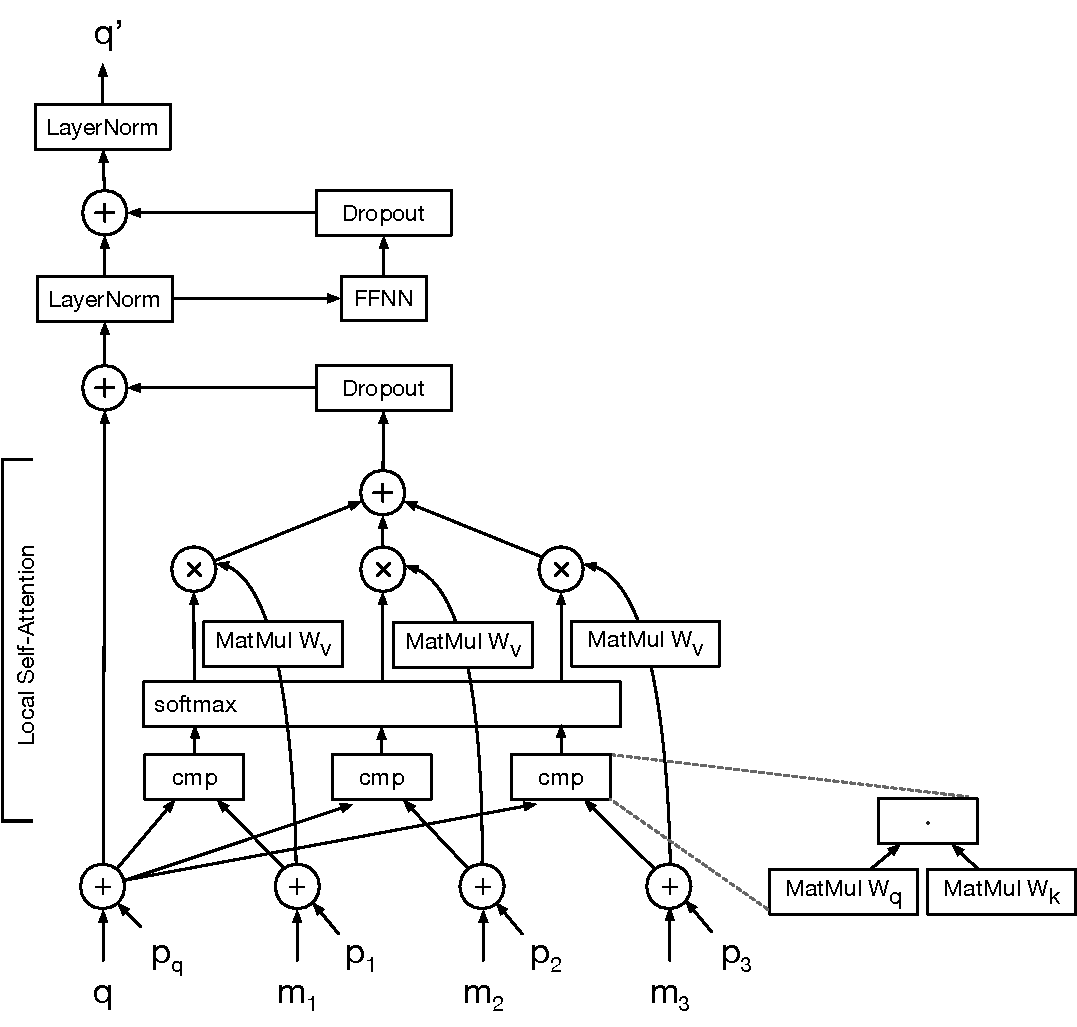
\includegraphics[scale=0.44]{ImageTransformerDiagram.pdf}
  \caption{A slice of one layer of the Image Transformer, recomputing the representation $q'$ of a single channel of one pixel $q$ by attending to a memory of previously generated pixels $m_1, m_2, \ldots$. After performing local self-attention we apply a two-layer position-wise feed-forward neural network with the same parameters for all positions in a given layer. Self-attention and the feed-forward networks are followed by dropout and bypassed by a residual connection with subsequent layer normalization. The position encodings $p_q, p_1, \ldots$ are added only in the first layer.}
  \label{fig:model-arch}
\end{figure}

For image-conditioned generation, as in our super-resolution models, we use an encoder-decoder architecture. The encoder generates a contextualized, per-pixel-channel representation of the source image.
The decoder autoregressively generates an output image of pixel intensities, one channel per pixel at each time step. While doing so, it consumes the previously generated pixels and the input image representation generated by the encoder. For both the encoder and decoder, the Image Transformer uses stacks of self-attention and position-wise feed-forward layers, similar to \citep{aiayn}. In addition, the decoder uses an attention mechanism to consume the encoder representation. For unconditional and class-conditional generation, we employ the Image Transformer in a decoder-only configuration.

Before we describe how we scale self-attention to images comprised of many more positions than typically found in sentences, we give a brief description of self-attention.

% Our generated images contain $3072$ positions ($\height=32$, $\width=32$, and $3$ channels) and computing attentions over all positions for the decoder is computationally expensive. We only use encoders for super-resolution where the images are of size $[8, 8, 3]$ (Section~\ref{sec:super-res}), allowing us to run full self-attention efficiently. Before we present our solutions to dealing with decoder self-attentions for images, we briefly describe the self-attention layer used in the Transformer.

Each self-attention layer computes a $\modeldim$-dimensional representation for each position, that is, each channel of each pixel. To recompute the representation for a given position, it first compares the position's current representation to other positions' representations, obtaining an attention distribution over the other positions. This distribution is then used to weight the contribution of the other positions' representations to the next representation for the position at hand.


Equations \ref{eqn:self-attention} and \ref{eqn:FFNN} outline the computation in our self-attention and fully-connected feed-forward layers; Figure \ref{fig:model-arch} depicts it. $W_1$ and $W_2$ are the parameters of the feed-forward layer, and are shared across all the positions in a layer.  These fully describe all operations performed in every layer, independently for each position, with the exception of multi-head attention. For details of multi-head self-attention, see \citep{aiayn}.

% \begin{equation}
% \query'= q + \mathrm{dropout}(\mathrm{layernorm}(\mathrm{FFNN}(\mathrm{softmax}\left( \frac{ W_{\query} \query (M W_{\key})^T }{\sqrt{d}} \right) M W_{\val})))
%  \label{eqn:self-attention}
% \end{equation}

% \begin{equation}
% \begin{split}
% \query' & =  \mathrm{layernorm}(q + \mathrm{dropout}(\mathrm{FFNN}( \\
% & \mathrm{softmax}\left( \frac{ W_{\query} \query (M W_{\key})^T }{\sqrt{d}} \right) M W_{\val}))) 
%  \label{eqn:self-attention}
% \end{split}
% \end{equation}

\begin{multline}
\query_{a} = \mathrm{layernorm}(q + \mathrm{dropout}( \\ 
\mathrm{softmax}\left(\frac{W_{\query} \query (M W_{\key})^T }{\sqrt{d}} \right) M W_{\val}))
\label{eqn:self-attention}
\end{multline}

\begin{equation}
\query' = \mathrm{layernorm}(\query_{a} + \mathrm{dropout} (W_1 \mathrm{ReLu}(W_2 \query_{a})))
\label{eqn:FFNN}
\end{equation}


%\sidenote{trandustin: do we want to mention the parameter/compute ratio and how we set that here (and/or in experiments)?}
In more detail, following previous work, we call the current representation of the pixel's channel, or position, to be recomputed the query $q$. The other positions whose representations will be used in computing a new representation for $q$ are $m_1, m_2, \ldots$ which together comprise the columns of the memory matrix $M$.
Note that $M$ can also contain $q$. We first transform $q$ and $M$ linearly by learned matrices $W_q$ and $W_k$, respectively.

The self-attention mechanism then compares $q$ to each of the pixel's channel representations in the memory with a dot-product, scaled by $1/\sqrt{\modeldim}$. We apply the $\mathrm{softmax}$ function to the resulting compatibility scores, treating the obtained vector as attention distribution over the pixel channels in the memory. After applying another linear transformation $W_v$ to the memory $M$, we compute a weighted average of the transformed memory, weighted by the attention distribution. In the decoders of our different models we mask the outputs of the comparisons appropriately so that the model cannot attend to positions in the memory that have not been generated, yet.

To the resulting vector we then apply a single-layer fully-connected feed-forward neural network with rectified linear activation followed by another linear transformation. The learned parameters of these are shared across all positions but different from layer to layer.

As illustrated in Figure\ref{fig:model-arch}, we perform dropout, merge in residual connections and perform layer normalization after each application of self-attention and the position-wise feed-forward networks \citep{layernorm2016, srivastava2014dropout}.

The entire self-attention operation can be implemented using highly optimized matrix multiplication code and executed in parallel for all pixels' channels.

%Figure\ref{fig:model-arch} depicts a single query $\query$ attending to previously generated outputs at $\memory_1, \memory_2, \ldots$, which comprise the memory $M$. Note that the memory will include the representation at the query position as well. We linearly transform $\query$ by a learned matrix $W_{\query}$, and compute compatiblities with each memory position $\memory_{i}$ linearly transformed by learned parameters $W_{\key}$, with a scaled dot product followed by a $softmax$. We compute a weighted average of the  memories transformed by another learned matrix $W_{\val}$, with the compatilibiliy weights to produce the output of self-attention at the query position. In decoder self-attention, We mask the compatibilities appropriately so that pixels cannot attend to that have not been generated. 

%Mathematically,

%In the next two sections, we will describe how we restrict our memories for faster training times.

\subsection{Local Self-Attention}
\label{sec:local-self-attention}

The number of positions included in the memory $l_{m}$, or the number of columns of $M$, has tremendous impact on the scalability of the self-attention mechanism, which has a time complexity in $O(h \cdot w \cdot l_{m} \cdot \modeldim)$.

The encoders of our super-resolution models operate on $8\times8$ pixel images and it is computationally feasible to attend to all of their $192$ positions. The decoders in our experiments, however, produce $32\times32$ pixel images with $3072$ positions, rendering attending to all positions impractical.

Inspired by convolutional neural networks we address this by adopting a notion of locality, restricting the positions in the memory matrix $M$ to a local neighborhood around the query position. Changing this neighborhood per query position, however, would prohibit packing most of the computation necessary for self-attention into two matrix multiplications - one for computing the pairwise comparisons and another for generating the weighted averages. To avoid this, we partition the image into query blocks and associate each of these with a larger memory block that also contains the query block. For all queries from a given query block, the model attends to the same memory matrix, comprised of all positions from the memory block.
The self-attention is then computed for all query blocks in parallel.
The feed-forward networks and layer normalizations are computed in parallel for all positions.

In our experiments we use two different schemes for choosing query blocks and their associated memory block neighborhoods, resulting in two different factorizations of the joint pixel distribution into conditional distributions. Both are illustrated in Figure~\ref{fig:conditional-factorizations}.

%, where the $O(n^2 \cdot \modeldim)$ complexity of full self-attention would slow down training times significantly for our decoder layers, as compared to machine translation. To combat this, we take an approach similar to convolutional neural networks where we restrict the memory positions to a local neighborhood around the query. We experiments with two approaches for local self-attention, shown in figure~\ref{fig:conditional-factorizations}:

\paragraph{1D Local Attention} \label{sec:loc-1d} 
For 1D local attention (Section~\ref{sec:loc-1d}) we first flatten the input tensor with positional encodings in raster-scan order, similar to previous work \citep{PixelRNN}. To compute self-attention on the resulting linearized image, we then partition the length into non-overlapping query blocks $Q$ of length $l_{q}$, padding with zeroes if necessary. While contiguous in the linearized image, these blocks can be discontiguous in image coordinate space. For each query block we build the memory block $M$ from the same positions as $Q$ and an additional $l_{m}$ positions corresponding to pixels that have been generated before, which can result in overlapping memory blocks.

\paragraph{2D Local Attention} \label{sec:loc-2d} In 2D local attention models, we partition the input tensor with positional encodings into rectangular query blocks contiguous in the original image space. We generate the image one query block after another, ordering the blocks in raster-scan order. Within each block, we generate individual positions, or pixel channels, again in raster-scan order.

As illustrated in the right half of Figure~\ref{fig:conditional-factorizations}, we generate the blocks outlined in grey lines left-to-right and top-to-bottom. We use 2-dimensional query blocks of a size $l_q$ specified by height and width $l_q = w_q \cdot h_q$, and memory blocks extending the query block to the top, left and right by $h_m$, $w_m$ and again $w_m$ pixels, respectively.

In both 1D and 2D local attention, we mask attention weights in the query and memory blocks such that positions that have not yet been generated are ignored.

As can be seen in Figure~\ref{fig:conditional-factorizations}, 2D local attention balances horizontal and vertical conditioning context much more evenly. We believe this might have an increasingly positive effect on quality with growing image size as the conditioning information in 1D local attention becomes increasingly dominated by pixels next to a given position as opposed to above it. 

%Even when generating $32\times32$ pixel images, however, we observe a significant improvement in negative log-likelihood when using 2D local attention in super-resolution, as shown in Table \ref{tab:superres_table}.


%shapes $[h_{\q}, w_{\q}]$, and memory blocks specified by offsets $[h_{\memory}, w_{\memory}]$. The memory region extends beyond the query block left, top-left, top, and top-right. Each position in the query can attend to every position in the query region that has been generated before and all the positions outside that also fall in the memory block. In the right figure, the query in the dashed box can attend to the unfilled pixels in the green region. We follow a similar procedure as local 1-attention, partitioning the $[\height, \width \times 3, \modeldim]$ tensor into query blocks and computing attention with their associated memory blocks in parallel, combining the results back into a tensor of the same shape.


\begin{figure}
%   \centering
  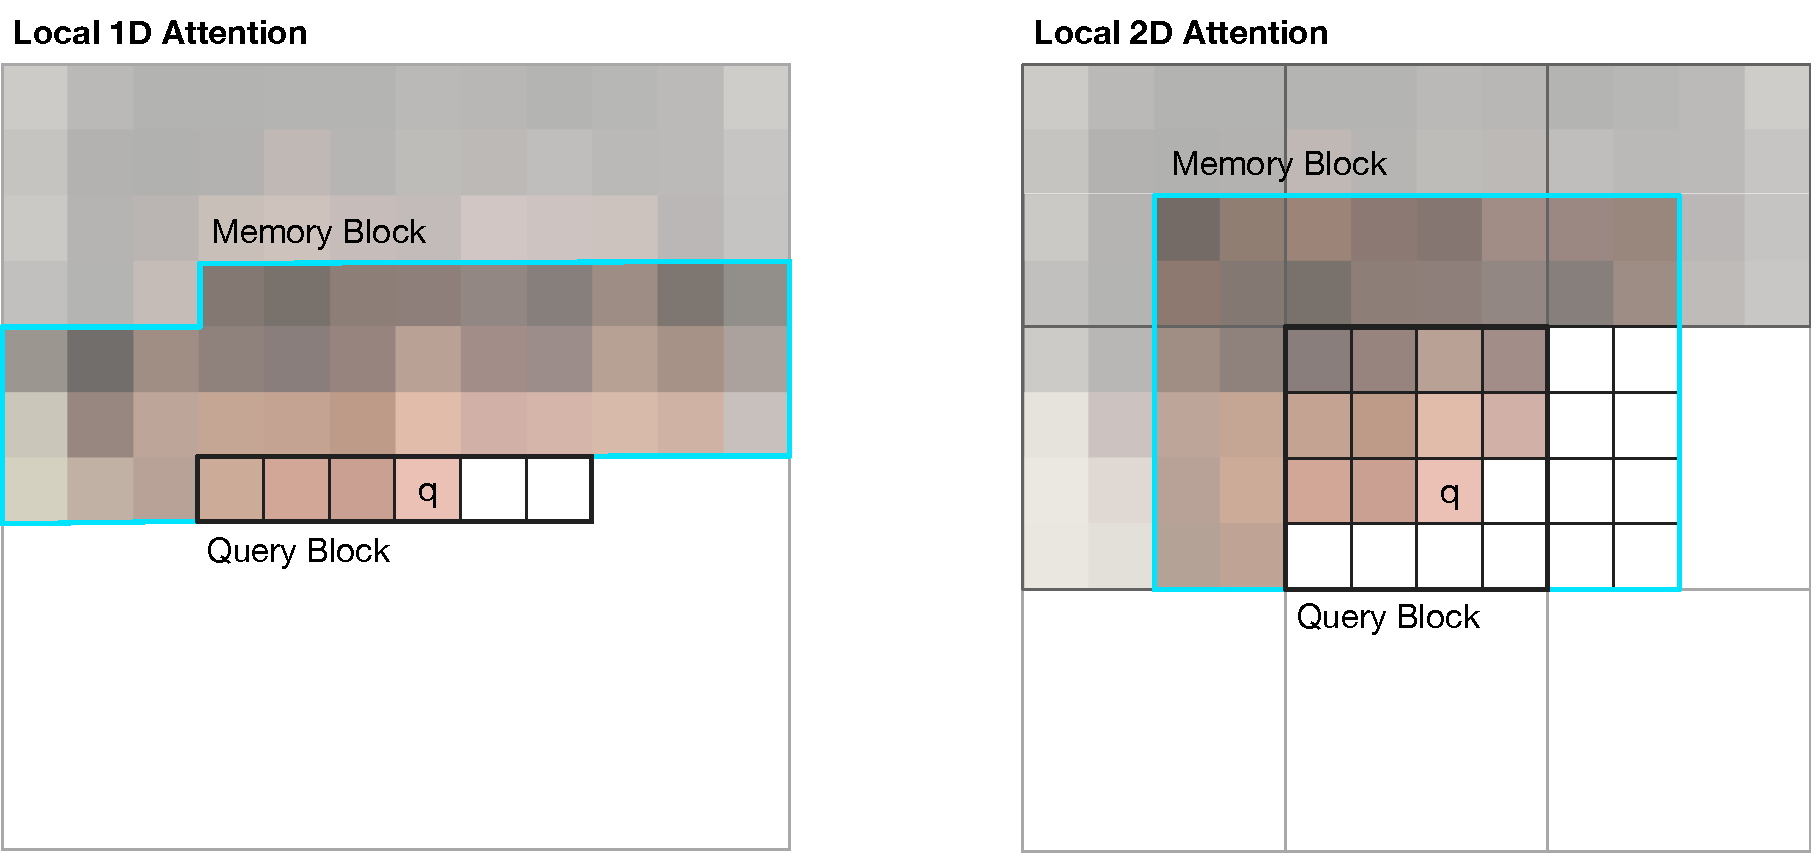
\includegraphics[scale=0.265]{ConditionalFactorizations.pdf}
  \caption{The two different conditional factorizations used in our experiments, with 1D and 2D local attention on the left and right, respectively. In both, the image is partitioned into non-overlapping query blocks, each associated with a memory block covering a superset of the query block pixels.
  In every self-attention layer, each position in a query block attends to all positions in the memory block.
  The pixel marked as $q$ is the last that was generated. All channels of pixels in the memory and query blocks shown in white have masked attention weights and do not contribute to the next representations of positions in the query block. While the effective receptive field size in this figure is the same for both schemes, in 2D attention the memory block
  contains a more evenly balanced number of pixels next to and above the query block, respectively.}
  \label{fig:conditional-factorizations}
\end{figure}

% \subsection{Local 1-d Attention} \label{sec:loc-1d}
% In local 1D attention, we treat the image as a flattened sequence of RGB values for each pixel as read in rastor scan order. The total length of a sequence becomes huge to be able to do full self attention. To be able to generalize to long sequences, we divide the $\query$ and $\memory$ into blocks
% \subsection{Local 2-d Attention} \label{sec:loc-2d}

% \subsection{Two-Dimensional Self-Attention}
% Self-attention in twice the dimensions!

\subsection{Loss Function}
\label{sub:loss}

We perform maximum likelihood, in which we maximize $\log p(x) = \sum_{t=1}^{h\cdot w\cdot 3} \log p(x_t\mid x_{<t})$ with respect to network parameters, and where the
% via stochastic gradient descent. 
network outputs all parameters of the autoregressive distribution.
%
We experiment with two settings of the distribution: a categorical distribution across each channel \citep{PixelRNN} and a mixture of discretized logistics over three channels \citep{PixelCNNpp}.

The categorical distribution (\emph{cat}) captures each intensity value as a discrete outcome and factorizes across channels. In total, there are $256\cdot 3=768$ parameters for each pixel; for $32\times 32$ images, the network outputs $786,432$ dimensions.
%
% For each pixel,
% \begin{equation*}
% p(x_{\rm rgb}\mid x_{<})
% =
% \operatorname{Categorical}(x_{\rm r})
% \operatorname{Categorical}p(x_{\rm g}\mid x_{\rm r})
% \operatorname{Categorical}p(x_{\rm b}\mid x_{\rm b})
% \end{equation*}
% This captures all possible values but can be slow to train, as there is no knowledge of ``closeness'' between intensities, where knowledge about intensity value 127 should assist in intensity value 128.

Unlike the categorical distribution, the discretized mixture of logistics (\emph{DMOL}) captures two important properties: the ordinal nature of pixel intensities and simpler dependence across channels \citep{PixelCNNpp}.
% In addition, it forgoes arbitrary factorization across pixel channels and uses a simple linear parameterization, where 
For each pixel, the number of parameters is $10$ times the number of mixture components: $10$ for one unnormalized mixture probability, three means,
% $\alpha_{r,g,b}$
% (one per channel), 
three standard deviations,
% $\sigma_{r,g,b}$ 
% (one per channel),
and three coefficients 
% $\beta_{1,2,3}$ 
which capture the linear dependence.
For 10 mixtures, this translates to $100$ parameters for each pixel; for $32\times 32$ images, the network outputs $102,400$ dimensions, which is a 7x reduction enabling denser gradients and lower memory.
% [This enables sparse gradients for faster training, memory, simpler factorization]
% \begin{align*}
% p(x_{\rm rgb}\mid \cdot)
% &=
% p(x_{\rm r}\mid \cdot)
% p(x_{\rm g}\mid x_{\rm r}, \cdot)
% p(x_{\rm b}\mid x_{\rm r}, x_{\rm g}, \cdot)
% \\
% \mu_r &= \alpha_r \\
% \mu_g &= \alpha_g + \beta_1 x_{\rm r} \\
% \mu_b &= \alpha_b + \beta_2 x_{\rm g} + \beta_3 x_{\rm g}.
% \end{align*}
